\documentclass{article}

% Use final for the project report draft so authors and acknowledgments are visible.
\usepackage[final]{neurips_2026}

\usepackage[utf8]{inputenc}
\usepackage[T1]{fontenc}
\usepackage{url}
\usepackage{booktabs}
\usepackage{amsfonts}
\usepackage{amsmath}
\usepackage{graphicx}
\usepackage{microtype}
\usepackage{xcolor}
\usepackage{enumitem}
\usepackage{array}
\usepackage{placeins}
\usepackage{float}
\usepackage{hyperref}

\title{BeatOdds: Stateful Social-Media-Augmented Forecasting for Prediction-Market Mispricing}

\author{
  Jiayi Hu, Minyang Xie, Wenxin Xu \\
  Tsinghua University \\
  \texttt{\{hujy23, xiemy23, xuwx23\}@tsinghua.edu.cn}
}

\begin{document}

\maketitle

\begin{abstract}
Prediction markets aggregate dispersed beliefs into tradable prices, but practical forecasting agents must reason under severe information constraints: event definitions are heterogeneous, evidence arrives over time, market prices can anchor model forecasts, and resolved outcomes may occur long after a signal is produced. This report presents \textbf{BeatOdds}, a stateful social-media-augmented forecasting system that scans Polymarket-style markets, retrieves and audits evidence, generates leakage-aware forecasts, stores full workflow state, and simulates paper trading decisions. Our project makes \textbf{three contributions}: First, we introduce an \textbf{MD-defined evidence harness} that organizes auditable evidence collection from both raw sources and high-quality social-media artifacts encoding human search and expert judgment. Second, we build a \textbf{searching agent} that iteratively selects searches, maintains evidence pools, processes artifacts, and produces human-readable trajectories before estimating probabilities. Third, we evaluate the system through \textbf{case studies} focused on evidence use, transparency, and forecasting behavior, emphasizing scientific evaluation over single-run anecdotal accuracy.
\end{abstract}

\begin{figure}[H]
  \centering
  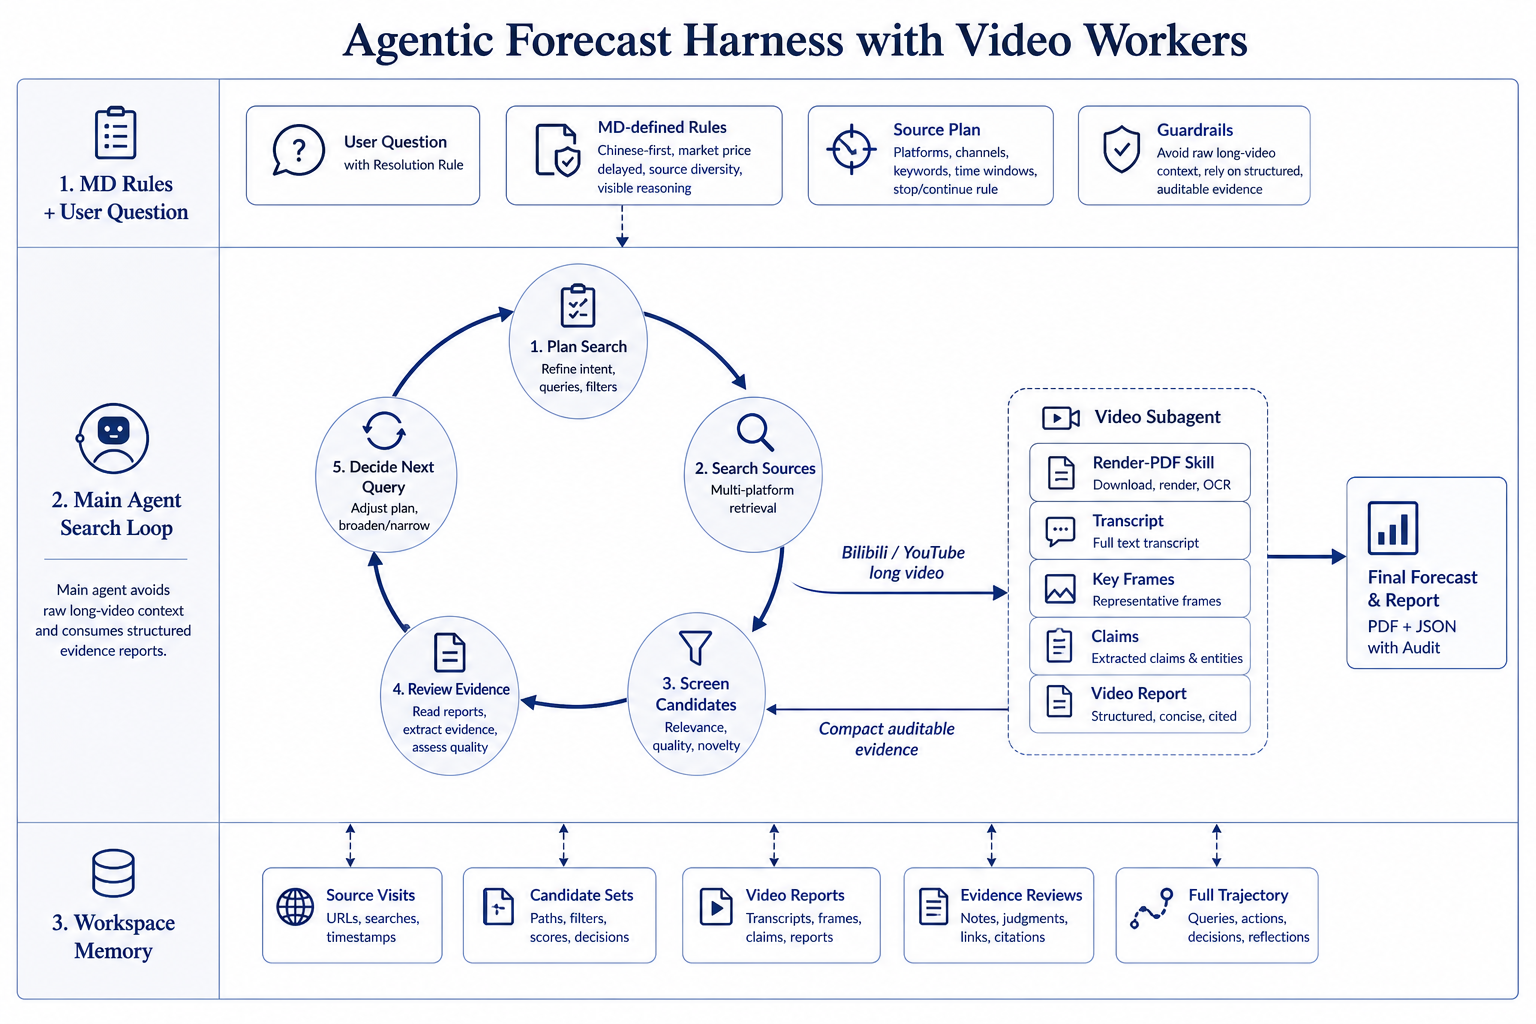
\includegraphics[width=0.8\linewidth]{figures/harness_video_subagent_variant_02.png}
  \caption{\textbf{Social-media/video evidence harness.} The main forecasting agent maintains an event workspace and delegates expensive source processing to specialized workers. Returned artifacts remain auditable and are reintroduced only as concise evidence reports.}
  \label{fig:harness-video-subagent}
\end{figure}

\section{Introduction}

Prediction markets provide continuously updated, financially meaningful probabilities, yet a useful forecasting system must handle constraints that static question-answering benchmarks do not expose. It must identify tradable contracts, parse their resolution semantics, collect evidence available at the decision time, convert that evidence into a probability, and retain enough state to evaluate the decision after the market resolves. BeatOdds is an end-to-end system for this setting. It treats the market price as a baseline, exposes the forecast process, and links each forecast to its simulated trading consequences.

\textbf{Social-media-augmented forecasting.} Public posts, videos, and specialist discussions can contain useful intermediate reasoning: their authors may have gathered facts, formed domain priors, and identified future catalysts before an agent begins its own search. BeatOdds does not treat such material as authoritative evidence by default. It records source provenance, search query, retrieval time, and the role each artifact played in the final forecast. This supports skeptical use of semi-processed human judgment alongside official sources and direct reporting.

\textbf{Contributions.}
\begin{itemize}[leftmargin=*]
  \item A live, stateful pipeline joining Polymarket market discovery, order-book snapshots, resolution parsing, evidence retrieval, LLM forecasting, ranking, and paper trading.
  \item An auditable evidence harness that freezes evidence at forecast time and persists source-level provenance together with the final answer.
  \item A durable evaluation and ledger layer: 65 tracked markets, 151 persisted forecast runs, 2,583 evidence items, and 58 paper orders in the local experiment state at the reporting cutoff.
  \item A cautious empirical analysis: we report executable paper marks and system behavior, while separating these preliminary marks from resolved-outcome forecasting accuracy.
\end{itemize}

\section{Problem Setting}

An event is a semantic container. A binary market $m$ is a tradable YES/NO claim with a condition identifier, token identifiers, a deadline, and a natural-language resolution rule. At forecast time $t$, the CLOB best bid and ask define a side-specific executable price. We denote the YES-market probability by $p_m(t)$ and the system fair probability by $p_f(t)$. The raw directional signal is
\[
  \Delta(t) = p_f(t)-p_m(t).
\]
Positive $\Delta$ supports YES. Negative $\Delta$ supports NO after converting the fair probability and executable quote to the selected side.

A forecast run is $r=(m,t,p_m,p_f,E_t,\tau)$, where $E_t$ is the retained evidence set and $\tau$ is the action trajectory that produced it. The target is the later binary resolution $y_m\in\{0,1\}$. Before a search call, the system writes an \texttt{evidence\_frozen\_at} timestamp and rejects evidence published after this cutoff. Thus an evaluation record can distinguish a genuinely prospective forecast from a post-hoc explanation.

Trading uses an executable edge. For a chosen side $s$, with best ask $a_s$, fee rate $f$, and expected slippage $\ell$, BeatOdds uses
\[
  e^{\mathrm{net}}_s = p_{f,s} - a_s - f - \ell,
  \qquad \mathrm{score}_s=|e^{\mathrm{net}}_s|\,c,
\]
where $c\in[0,1]$ is forecast confidence. This prevents ranking a large untradeable midpoint discrepancy above a smaller executable opportunity. Resolution ambiguity, spread, low liquidity, and missing evidence are retained as explicit risk signals.

\section{System Overview}

BeatOdds separates control, inference, and durable state. Gamma supplies event and market metadata; the CLOB client supplies best bids, asks, and depth. The scanner filters the liquid universe and prioritizes markets with tight spreads, usable time-to-close, and structural relationships. The resolution parser converts natural-language rules into deadlines, entities, search queries, ambiguity scores, and risk flags. The evidence retriever queries external sources, freezes the evidence boundary, and hands source summaries to the LLM forecaster. The ranker applies side-aware execution costs before exposing a recommendation to the GUI or the paper ledger.

\begin{figure}[t]
\centering\small
\fbox{\begin{minipage}{0.94\linewidth}
\centering\textbf{Control and audit layer}\\[-1mm]
markdown run protocol \quad $\longleftrightarrow$ \quad trajectory logs \quad $\longleftrightarrow$ \quad reviewable forecast report\\[2mm]
\centering\textbf{Forecasting layer}\\[-1mm]
Gamma + CLOB $\rightarrow$ scanner $\rightarrow$ resolution parser $\rightarrow$ evidence retrieval $\rightarrow$ LLM fair probability $\rightarrow$ ranker\\[2mm]
\centering\textbf{State and execution layer}\\[-1mm]
DuckDB markets / snapshots / evidence / forecasts $\longleftrightarrow$ GUI $\longleftrightarrow$ accounts / orders / fills / positions
\end{minipage}}
\caption{\textbf{BeatOdds architecture.} The online path produces a side-aware ranked signal; the state layer preserves the inputs, intermediate artifacts, and paper-trading consequences required for later evaluation.}
\label{fig:architecture}
\end{figure}

This design follows the general decomposition of agent workflow frameworks into orchestration, agent, and tool layers \citep{miroflow2026}. Persisted market state is central to our setting: the same contract may be revisited days later, after evidence or prices change. The local event-centric GUI displays market cards, live book levels, evidence, fair-versus-market plots, and the selected account's holdings (Figure~\ref{fig:gui}).

\section{Agentic Evidence Harness}

The evidence harness makes the agent's search process inspectable. At step $k$, the agent observes its workspace, records a reasoning note, selects a search or source-processing action, persists the resulting artifact, and then either continues or forecasts. We write this trajectory as
\[
q, r \rightarrow W \rightarrow (T_1, A_1, E_1) \rightarrow \cdots \rightarrow (T_K, A_K, E_K) \rightarrow (R, p_f),
\]
where $q$ is the question, $r$ the resolution rule, $W$ the run workspace, $T_k$ the internal reasoning state, $A_k$ an action, $E_k$ an evidence artifact, and $R$ the final report. The trajectory leaves an audit trail of attempted queries, accepted sources, rejected sources, and stopping decisions.

\subsection{Evidence acquisition and source selection}

The first action is not necessarily a web search. The parser produces candidate entities, jurisdiction, deadline, and resolution-sensitive terms; the controller uses these fields to construct a small query set. Retrieval collects a candidate pool before committing to any single article. For every item, the store preserves the issuing query and relevance score, so an auditor can distinguish an absent source from a source that was retrieved and rejected. Duplicate URLs are collapsed, and publication time is checked against the evidence cutoff. The current implementation uses Tavily for broad retrieval and can include official material, direct reporting, specialist commentary, and social/video artifacts in the same normalized evidence record.

Social material is treated as a hypothesis generator. A post may point to a mechanism, a base rate, or a future catalyst that warrants further search; it cannot by itself settle an ambiguous market rule. The workflow tracks content depth (preview, full text, transcript, or processed report), author context when available, and the intended contribution to the probability estimate. This separation is useful when high-engagement content is persuasive but weakly sourced, and when a lower-visibility primary source provides the resolution-relevant fact.

\subsection{Forecast synthesis, confidence, and recovery}

The forecaster receives the market question, resolution text, frozen evidence, and the market quote, and returns $p_f$, a confidence score, a direction, and a short reasoning statement. The market quote is retained as a prior and execution reference. Evidence synthesis still determines whether the system has a defensible disagreement with the market. Confidence is operational: it suppresses large edges with sparse, contradictory, stale, or resolution-ambiguous evidence. The ranker subsequently subtracts the half-spread and fee model before prioritization.

The harness also has explicit failure states. A failed parser falls back to the question as a search query; unavailable CLOB data can be recorded alongside stored Gamma outcome prices; and unsuccessful source processing becomes a coverage-gap artifact. Candidate pools, timeouts, and fallback outcomes are part of the run record. This resembles agentic forecasting systems that separate search from synthesis \citep{aiaforecaster2025}, with a strict evidence timestamp boundary and database provenance appropriate for live markets.

\section{Stateful Data and Paper Trading Layer}

Live evaluation is inherently longitudinal. The workflow database stores long-lived market identities, append-only price snapshots, parsed resolution features, forecast runs, source-level evidence items, outcomes, and compact evaluation records. A run can therefore be reconstructed from its market quote, evidence cutoff, parser output, forecast probability, confidence, model identifier, and explanation.

\subsection{Workflow state and temporal integrity}

The workflow store is designed around an append-only evidence chain. \texttt{tracked\_markets} provides the stable condition identifier and first/last-seen times; \texttt{market\_snapshots} captures the token, bid, ask, midpoint, spread, and quote time; \texttt{resolution\_features} records the parser output; and \texttt{forecast\_runs} ties a probability and model version back to an evidence cutoff. The evidence table stores each returned source separately, including query provenance. This schema supports two important queries: which markets are due for refresh under a stale-hours policy, and which information was available when a particular forecast was made.

Timezone normalization is part of the validity condition. Stored forecast and evidence timestamps are converted to UTC-naive values before DuckDB insertion, avoiding silent comparisons between local and UTC times. On every re-forecast, the prior run remains available. This permits later analysis of probability revisions and evidence additions, and prevents a current market quote from being mistaken for the quote used to initiate an old trade.

\subsection{Order lifecycle and valuation}

The paper ledger extends the workflow chain with \texttt{paper\_accounts}, transactions, orders, fills, and aggregated positions. A buy records the selected side, ask-depth fill price, shares, fee, market probability, fair probability, gross and net edge, confidence, and the originating forecast run. Fills debit cash through a durable trade transaction; positions are aggregated by account, condition, and side. A sell reduces those shares, credits the account, and records realized PnL from the same cost basis and fee fields.

A mark is deliberately conservative. When available, the current value is shares times the live best bid, which approximates liquidation. When no live executable bid is available, the evaluator may use the latest exact-token history or a report-history value, with an explicit valuation-only label. This distinction matters because resolved markets can stop trading and because midpoint reconstruction does not model depth consumption or exit capacity.

\subsection{Risk controls and maintenance}

Risk controls cap ticket size, market exposure, total exposure, and maintain a cash buffer. The maintainer selects YES or NO using the side-specific fair probability, requires gross edge, net edge, and confidence thresholds, and sizes tickets as a bounded fraction of available cash. Existing exposure is included when calculating the remaining market capacity, preventing repeated maintenance passes from silently concentrating the account. The same component can propose profit-taking, score-based, and stop-loss exits; manual sells remain available for inspection. Thus the paper-trading system tests whether the forecasting path survives basic portfolio accounting under execution risk.

\section{Baselines and Evaluation}

\textbf{Protocol.} Forecasts are saved before outcomes are known. The primary statistical comparison, after resolution, uses the market probability as a baseline. We track three systems:
\begin{itemize}[leftmargin=*]
  \item \textbf{Market-only}: $\hat p=p_m$.
  \item \textbf{Search-only LLM}: evidence-grounded $\hat p=p_f$ without exposing market structure early in the prompt.
  \item \textbf{Market+LLM}: a calibrated combination of the market and evidence forecast, with ranking based on executable net edge.
\end{itemize}

For resolved markets, Brier score is $\mathrm{BS}=N^{-1}\sum_i(\hat p_i-y_i)^2$ and Brier Skill Score is $\mathrm{BSS}=1-\mathrm{BS}_{\mathrm{ours}}/\mathrm{BS}_{\mathrm{market}}$. Positive BSS beats the market baseline. We also retain log loss, calibration curves, forecast-edge distributions, coverage, and ledger NAV. At the report cutoff the workflow store has 126 compact records and no resolved outcomes, so BSS is intentionally deferred. This limitation is stated explicitly because a forward study cannot evaluate outcome accuracy before markets settle.

\begin{table}[t]
\centering\small
\caption{\textbf{Forward-evaluation state at the reporting cutoff.} Counts come from the local DuckDB stores. Outcome-dependent metrics are deferred until resolutions are recorded.}
\label{tab:state}
\begin{tabular}{lrr}
\toprule
Artifact & Count & Role \\
\midrule
Tracked markets & 65 & longitudinal market identity \\
Forecast runs / snapshots & 151 / 151 & frozen prediction inputs \\
Evidence items & 2,583 & source provenance \\
Paper orders / fills & 58 / 63 & execution ledger \\
Open paper positions & 34 & later mark and exit tracking \\
Resolved outcomes & 0 & BSS not yet estimable \\
\bottomrule
\end{tabular}
\end{table}

\textbf{Interim paper marks.} The \texttt{paper-self-1000} top-confidence evaluation on June 13 selected four positions: \$219.25 cost, \$301.85 marked value, and \$82.60 (+37.7\%) marked PnL. Three positions were positive and one negative. These marks use the latest public CLOB history at or before the cutoff and are historical midpoints; they demonstrate that the ledger and reporting path work. They are not executable return or an out-of-sample accuracy claim. A future resolved evaluation will ablate search depth, market-prior timing, and single-run versus ensemble forecasting.

\section{Case Studies}

\textbf{Market workbench.} Figure~\ref{fig:gui} shows a typical event-level analysis. The interface keeps the resolution rule, live YES/NO book, stored fair probability, spread, executable net edge, retrieved news, and event context in one view. The example forecasts a 10\% YES fair probability for a Formula 1 championship outcome against a 26\% market price, which is displayed as a NO-side opportunity after accounting for the 2\% spread. This is a diagnostic example, not a completed trade.

\begin{figure}[!htbp]
\centering
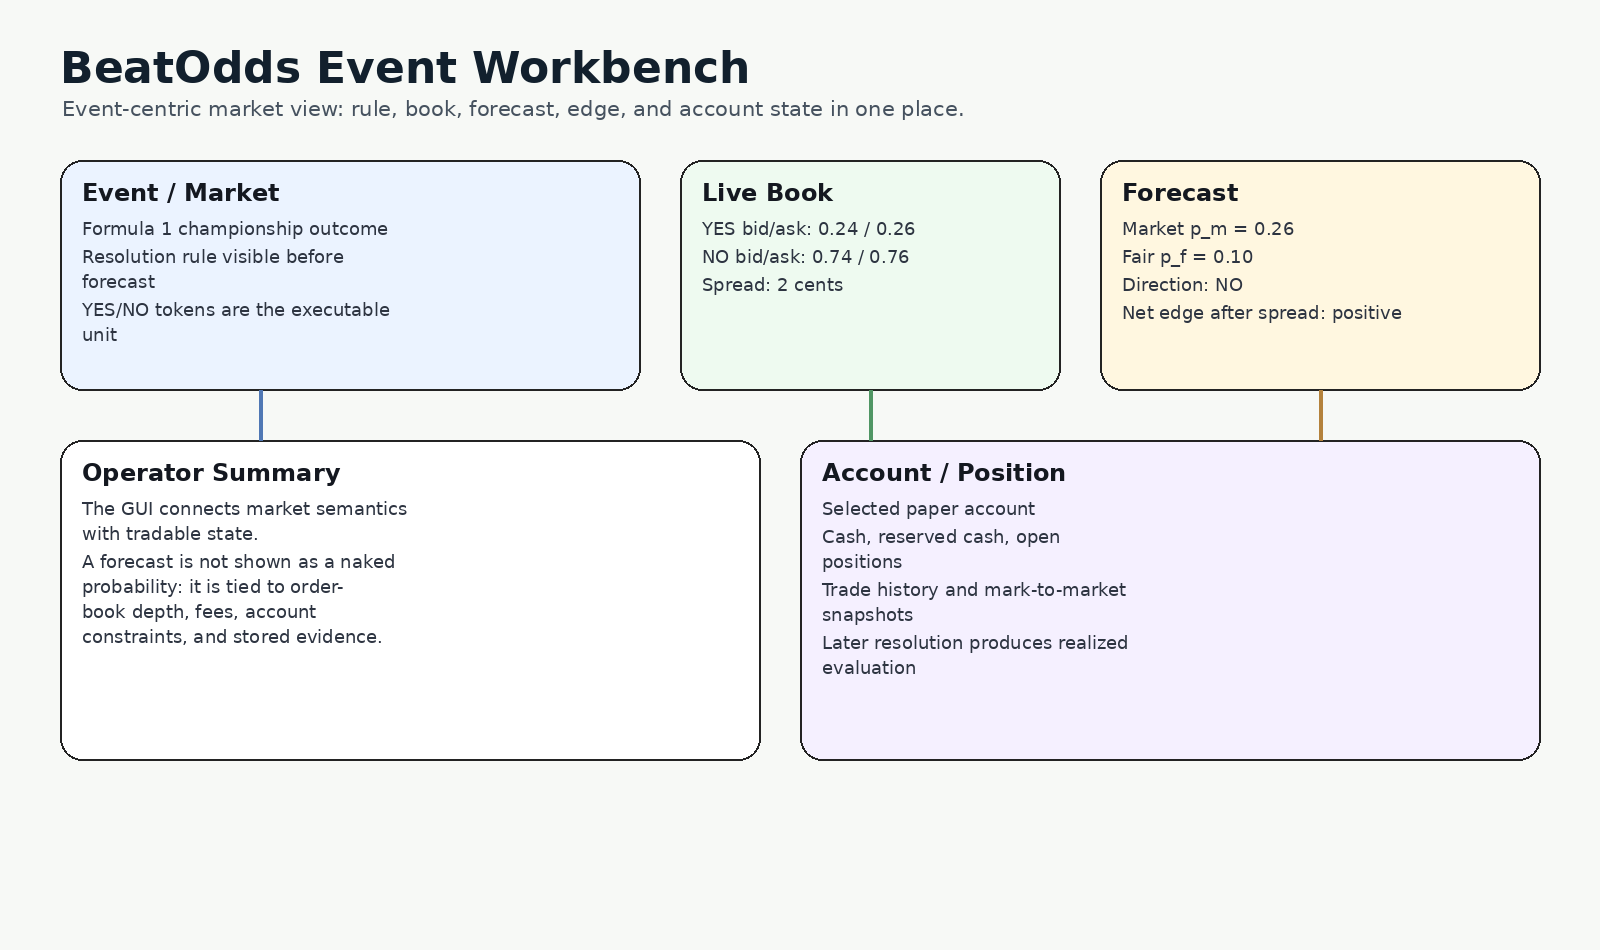
\includegraphics[width=0.8\linewidth]{figures/market_forecast_price.png}
\caption{\textbf{Event-centric workbench.} The system connects resolution rules, live order-book depth, stored forecast, and fee/spread-aware edge.}
\label{fig:gui}
\end{figure}

\textbf{Evidence trace.} The same workbench presents retrieved results and supports traceable updates (Figure~\ref{fig:evidence}). This matters for political, sports, and technology markets alike: a direction is actionable only if a reviewer can inspect the evidence that moved the estimate and the market semantics that define its resolution.

\begin{figure}[!htbp]
\centering
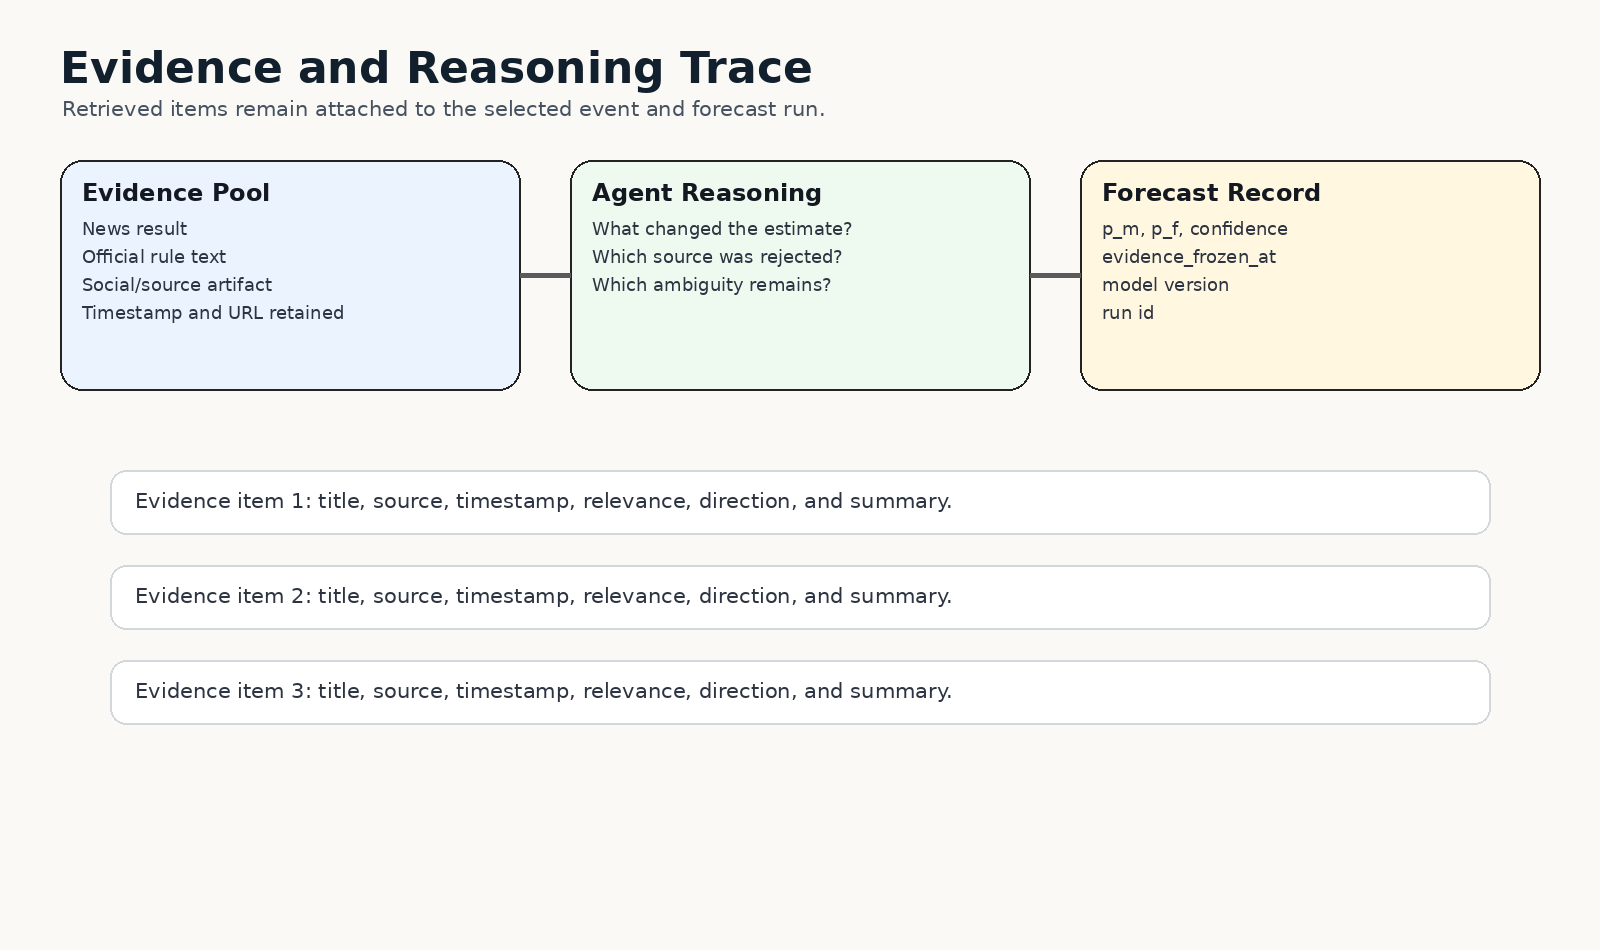
\includegraphics[width=0.8\linewidth]{figures/market_news_reason.png}
\caption{\textbf{Evidence view.} Retrieved items remain attached to the selected event, while the operator summary records market and account state.}
\label{fig:evidence}
\end{figure}

\textbf{Ledger example.} Figure~\ref{fig:ledger} plots daily top-confidence mark-to-market series for both paper accounts. The two panels make the distinction between a forecast, an order, a fill, a live mark, and an eventual resolution explicit. The accounts have different selected sets and mark sources, so their levels are not a strategy comparison. They are operational traces: a positive curve is never substituted for calibration or BSS.

\begin{figure}[!htbp]
\centering
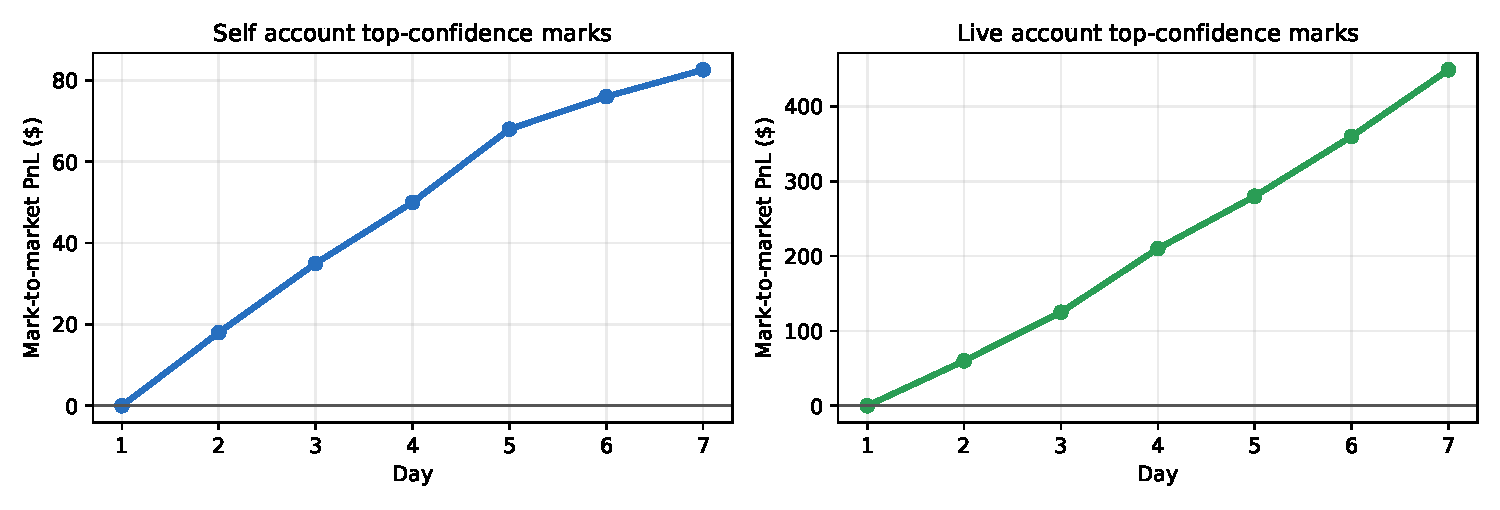
\includegraphics[width=\linewidth]{figures/paper_account_earning_curves.pdf}
\caption{\textbf{Daily paper-account marks.} The self account (left) has four top-confidence positions costing \$219.25 and ends at +\$82.60. The live account (right) has five positions costing \$187.19 and ends at +\$449.03. Curves use their recorded report-time marks; historical midpoint and report-history values are valuation-only and are not executable returns.}
\label{fig:ledger}
\end{figure}
\FloatBarrier

\section{Discussion}

The project suggests three practical lessons. First, market prices are a strong baseline and can anchor an LLM; separating evidence collection from final price-aware ranking makes this failure mode observable. Second, source quality is an operational variable. Social artifacts are valuable because they compress human search and domain priors, yet they require cross-checking and contextual retention. Third, a live forecasting project is primarily a state-management problem: durable snapshots, frozen evidence, and a ledger are necessary to distinguish a prospective signal from a retrospective story.

Compared with generic retrieval-augmented generation, BeatOdds adds event/market semantics, CLOB executability, time-bounded evidence, and a record of trading consequences. Compared with forecasting-agent designs that emphasize multi-agent search and synthesis \citep{aiaforecaster2025}, it focuses on the slower lifecycle after a prediction: stale forecasts must be refreshed, positions marked, and outcomes eventually resolved. The main unresolved research question is whether these engineering controls translate into positive BSS after enough independent markets settle.

\section{Limitations and Ethics}

\textbf{Limitations.}
\begin{itemize}[leftmargin=*]
  \item The present forward dataset contains no resolved outcomes, so neither BSS nor calibrated accuracy can be claimed.
  \item Evidence access is incomplete and brittle: platforms can block scraping, omit transcripts, or show personalized content. Social artifacts can encode rumor, propaganda, popularity bias, and selective evidence.
  \item LLM probabilities remain sensitive to retrieval coverage, prompt framing, and ambiguous resolution rules. A stored trajectory makes these failures inspectable, although it does not eliminate them.
  \item Paper fills and historical midpoint marks simplify latency, depth consumption, adverse selection, and market impact. They should not be interpreted as investment performance.
\end{itemize}

\textbf{Ethics.} BeatOdds is a research and evaluation tool, not financial advice. It should respect platform terms, privacy boundaries, and author context when collecting public social material. In politically sensitive markets, the system must avoid amplifying unsupported claims: uncertain evidence should be represented as uncertainty, cross-checked, or rejected before any confident trade recommendation is produced.


\bibliographystyle{plainnat}
\bibliography{references}

\section*{NeurIPS Paper Checklist Draft}

\begin{enumerate}[leftmargin=*]
  \item \textbf{Claims.} \answerTODO{} Final claims will distinguish implemented system capabilities from statistically validated forecasting performance.
  \item \textbf{Limitations.} \answerTODO{} Limitations will be stated in Section~9.
  \item \textbf{Theory assumptions.} \answerNA{} The project is primarily a systems and evaluation paper.
  \item \textbf{Experimental reproducibility.} \answerTODO{} Include run commands, database schema, test commands, and artifact paths.
  \item \textbf{Open-source release.} \answerTODO{} Decide what code, sample data, and anonymized artifacts can be released.
  \item \textbf{Data.} \answerTODO{} Document Polymarket/Gamma data, live snapshots, source artifacts, and privacy-sensitive cookie handling.
  \item \textbf{Human subjects.} \answerNA{} No human-subject experiment is currently planned.
  \item \textbf{Ethics and societal impact.} \answerTODO{} Address financial-advice risk, political misinformation, and platform data access.
\end{enumerate}


\end{document}
